% Plan:
%
% Spis treści
% Spis rysunków
% Słowniczek skrótów
%
% Wstęp (1-2 strony): geneza, obszar, zawartość, dokonania autorów, opis struktury pracy
%
% Rozdziały merytoryczne (4-5, zrównoważone objętościowo):
%   Preambuła (ok. 0.5 strony)
%   Punkty merytoryczne (4-6)
%   Podsumowanie rozdziału
%
%   * opis technologii i uzasadnienie wyboru do rozwiązania problemu
%   * analiza wymagań + projekt systemu (architektura)
%   * opis implementacji, sposób uruchomienia
%   * badania eksperymentalne (tutaj także: profiling, opóźnienia)
%
% Podsumowanie pracy / Zakończenie
%   Wnioski końcowe
%   Co się udało / nie udało (+dlaczego!)
%   Możliwości rozwoju
%
% Spis literatury (numerowany, w tekście _muszą_ być odniesienia, ~20 pozycji)
%
%
% INNE:
%   * całość - ok. 60-70 stron
%   * numeracja - nie więcej, niż 3-poziomowa


\documentclass[11pt]{book}
\usepackage[top=3cm, bottom=4cm]{geometry}
\usepackage[usenames,dvipsnames]{color}


% \usepackage[polish]{babel}
\usepackage[utf8]{inputenc}
\usepackage[T1]{fontenc}
\usepackage{fullpage}
\usepackage[pdfborder={0 0 0}]{hyperref}
\usepackage{float}
\usepackage{graphicx}
\usepackage{scrtime}
\usepackage{tabularx}
\usepackage{listings} 
\usepackage{caption}
\usepackage{color}
\usepackage{hyperref}
% \usepackage[toc,acronym]{glossaries}

\newcommand{\code}[1]{\begin{tt}{#1}\end{tt}}

\newcommand{\reqlabel}[1]{{\textcolor{Red}{\textbf{#1}}\label{#1}}}
\newcommand{\reqref}[1]{\hyperref[#1]{{\textcolor{Red}{\textbf{#1}}}}}

\newcommand{\tasklabel}[1]{{\textcolor{Blue}{\textbf{#1}}\label{#1}}}
\newcommand{\taskref}[1]{\hyperref[#1]{{\textcolor{Blue}{\textbf{#1}}}}}


\title{Component-based system for management of multilevel virtualization of networking resources}
\author{Robert Boczek \and Dawid Ciepliński}

\begin{document}

  \maketitle
    
  \tableofcontents

  \chapter*{Division of labour} %podzial pracy
	

  \chapter{Introduction}

    % QoS, rezerwacja zasobów, izolacja we współczesnych systemach informatycznych


  \chapter{Context}  % TODO ładniej

    \section*{Chapter overview}


    \section{QoS-aware networking}


    \section{Resource virtualization approaches}


    \section{Multilevel network virtualization}

      \subsection{Virtual network resources}

      \subsection{Fine-grained QoS control}

      \subsection{Virtual appliances}

      \subsection{,,Network in a box'' concept}


    \section{Applications and benefits of virtual infrastructures}

      \subsection{Testing and simulations}

      \subsection{Improving server-side infrastructure scalability}

      \subsection{Infrastructure as a service}

      \subsection{The role of resource virtualization in the SOA stack}


    \section*{Summary}


  \chapter{Requirements analysis}
    
    \section*{Chapter overview}

    \section{Functional requirements}

      \subsection{Instantiation}

      \subsection{Discovery}

      \subsection{Accounting}  % kz: raczej Monitoring


    \section{Non-functional requirements}

    \section{Underlying environment characteristics}

    \section{General approach and problems it imposes}

      \subsection{Load balancing / Deployment}

      \subsection{Infrastructure isolation}

      \subsection{Broadcast domain preservation}

      \subsection{Constraints}


    \section*{Summary}


  \chapter{Solaris OS as a resource virtualization environment}

    \section*{Chapter overview}

    \section{General information}

    \section{Lightweight OS-level virtualization with Solaris Containers}

    \section{Crossbow - network virtualization technology}

    \subsection{Crossbow architecture}

      One of the most important condition in terms of network virtualization is that network traffic
      should be insulated between virtual machines. This kind of isolation can be achieved by having
      a dedicated physical NIC, network cable and port from the switch to the virtual machine
      itself.  Moreover, switch must also ensure sustainability on every port. In every other case
      virtual machines will definitely interfere between each other.
 In a particular case when we
      have to share physical NIC between virtual machines the most promising solution is to
      virtualize NIC hardware and the second layer of the OSI/ISO stack where sharing is fair and
      interferences will be avoided. These approach was adapted in the Crossbow architecture in
      OpenSolaris OS.
 Traffic separation is achieved by fundamental blocks of new architecture
      which are Virtual NICs (VNICs) created by dividing NIC into many VNICs. 
 A VNIC can be
      created over NIC or Etherstub ( more about them later ) and be dynamically controlled by the
      bandwidth and CPU resources assigned to it.
 The crossbow architecture has introduced fully
      paralized network stack structure. Each stack could be seen as fully independent lane (without
      any shared locks, queues, and CPUs) therefore network isolation is guaranteed. Key concept is
      hardware classification performed by the NIC over which VNIC was created. Each lane has a
      dedicated buffer for Transmit (Tx) and Receive (Rx) ring. In case when load exceeds assigned
      limit packets must be dropped as it is wiser to dop them then to expend OS CPU resources. 

      
 \begin{figure}[H]
      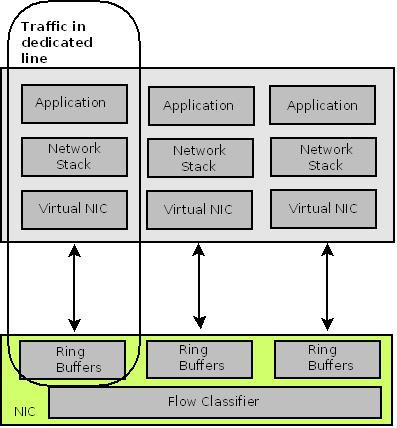
\includegraphics[width=\textwidth]{img/crossbow-traffic-dedicated-line.jpeg}
      \caption{Dedicated lines in the Crossbow architecture}
 \end{figure}
		
		\subsection{Virtualization lines}

      Virtualization is the most key component in the Crossbow architecture. Each lane consists some
			used to some concrete type of traffic. It usually would be composed of: 
			\begin{enumerate}
				\item{NIC resources( receive and transmit rings, interrupts, MAC address slots )}
				\item{Driver resources( DMA bindings )}
				\item{MAC layer resources ( data structures, execution threads, locks )}
			\end{enumerate}
			
			A virtualization lane can be one of two types, hardware-based or software-based.
			
			\subsubsection{Hardware-based virtualization lanes}
			
			This type requires ability to partitioning resources from NIC. The minimum requirement is that a hardware-based lane should must have a dedicated receive ring.
			Other resources such as transmit lane can be exclusive or shared between lanes. Each virtual machine could have one or more lanes assigned and the incoming packets
			would be distributed among them based on even scheduling unless some administrative polices where created, such as priority or bandwidth limit.		
			
			\subsubsection{Software-based virtualization lanes}
			
			In case when NIC runs out of hardware-based virtualization lane, receive and transmit rings may be shared by multiple VNICs. The number of software-based virtualization 
			lanes also often called softrings is unlimited. The main disadvantage of software-based lanes is the lack of fairness and isolation which in fact is provided in hardware-based
			lanes. The received and sent rings may work also in mix mode, whereas some of the rings may be assigned to software and some may be assigned to hardware based lanes.	
			
		\subsection{Dynamic polling}	
			
			The Crossbow architecture proposed two types of working mode. Currently used mode is determined by traffic and load. Under low load, where the rate of arraving packets is lower than
			time of packet processing, lane works in the interrupt mode which means that receive ring generates an interrupt when new packet arrives. However, when the backlog grows, the line 
			switches to dynamic polling mode in which a kernel thread goes down to the receive ring in the NIC hardware to extract all outstanding packets in a single chain. Key aspect is that 
			every virtualization lane works independently and transparently from each other. Usually only three threads are used per lane:
			
			\begin{enumerate}
				\item{Poll thread which goes to the NIC hardware to get all packet chain}
				\item{Woker thread which is responsible for protocol processing (IP and above) or delivers packets to virtual machine. Thread performs also any additional transmit work which is a natural 
				requirement some concrete protocol, such as processing TCP packets that require sending ACK packets.}
				\item{Transmit thread that is activated when if packets are being sent after transmit side flow control relief discharge, or after retreiving transmit descriptor. Application or virtual 
				machine can transmit any packets without performing queuing because of flow control or context switching.}
			\end{enumerate}

		
		\subsection{Crossbow elements}

			\subsubsection{VNics}
			Virtual NICs (VNICs) that are related to their own lane are the key element in crossbow architecture. There is no
			difference between NIC and VNIC in administration, they are all treated as data links. Every VNIC has an assigned
			lane and flow classifier which classifies received packets by VNIC's MAC address and sometimes by the VLAN tag.
			If created with a VLAN tag, protocols like GVRP or MVRP may be used to register the VLAN tag with the physical switches
			too.	

			In terms of sharing bandwidth, Crossbow enables administrative control of bandwidth for every single VNIC. The bandwidth of the link
			is implemented by regulating the periodic intake of incoming packets per dedicated lane. The network stack allows only as many packets as it was 
			assigned to specific VNIC. The lane picks more packets when the next period begins. In case of regulating the speed of transmited bandwidth it is much
			easier as the network stack can either control the application that is generating the stream of packets or just drop the excessive amount of packets.
			These mechanisms are also used in flows QoS described and discussed later in this paper.

			\subsubsection{Virtual switching}
			
			Virtual switches created always implicitly when the first VNIC is defined under existing NIC could never be accessed directly nor be visible by
			any user ( even administrator ). 
			
			\begin{figure}[H]
				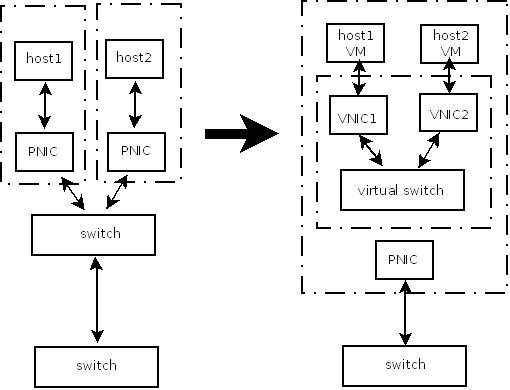
\includegraphics[width=\textwidth]{img/physical_and_virtual_switches_mapping.jpeg}
				\caption{Mapping between physical and virtual network building elements}
			\end{figure}
			
			Semantics assured by virtual switches are the same as provided by physical switches: 
			\begin{enumerate}
				\item{VNICs created on top of the same NIC can send ehterstub packets to each other}
				\item{Broadcast packets received by the underlying NIC are distributed to every single VNIC that was defined on the top of this NIC}
				\item{Broadcast packets sent by one of the VNICs is distributed to all VNICs defined on the top of the same NIC and to the NIC for further transmission as well}
				\item{In terms of multicast network traffic multicast group membership is monitored and used for distributing packets to appropriate VNIC}
			\end{enumerate}

			Connectivity between VNICs is available only when they were defined on the top of the same NIC. 

			\subsubsection{Etherstubs}

        As it was mentioned before, the MAC layer provides the virtual switching capabilities which allow VNICs to be created over existing physical NICs.
        In some cases, creating virtual networks without the use of a physical NIC is more welcomed than creating over physical NICs. In that case VNICs 
        would be defined on the top of pseudo NICs. The Crossbow provides these kind of elements which are called Etherstubs. These components could be used
        instead of NICs during creation of VNICs.
		
			\subsubsection{Examples}

        \textbf{dladm} is the admin command for managing NICs, VNICs and Etherstubs. Below we present a few examples of creating VNICs, Etherstbus and how
        to assigned bandwidth and priority to theses elements.

        \begin{enumerate}
        	\item{dladm create-vnic vnic1 -l e1000g0 - creates new VNIC \textbf{vnic1} over existing NIC \textbf{e1000g0}}
        	\item{dladm create-etherstub ether00 - creates new Etherstub \textbf{ether00}}
        	\item{dladm show-linkprop vnic11 - lists all properties assigned to \textbf{vnic11} link}
        	\item{dladm set-linkprop -pmaxbw=1000 vnic11 - assignes 1Mbps bandwith limit to \textbf{vnic11} link}
        	\item{dladm set-linkprop -ppriority=low vnic11 - assignes low priority to \textbf{vnic11} link}
        \end{enumerate}

        Here we have just presented some basic commands. For more examples see \textbf{man dladm}
        

    \section{Resource access control}

    \section*{Summary}
	


  \chapter{The system architecture}

    \section*{Chapter overview}

      The \nameref{sec:domain-model} section describes the transformations performed by the system's components in order to instantiate/deploy an object model. These include simple one-node instantiation as well as more complex multi-node instantiations.

      % tutaj tez kilka slow i JIMSie i integracji + co to daje


    \section{High-level design}


    \section{System components and their responsibilities}

      \subsection{Assigner}

      \subsection{Supervisor}

      \subsection{Worker}


    \section{Crossbow resources instrumentation}


    \section{Domain model and data flows} \label{sec:domain-model}


    \section*{Summary}


  \chapter{Implementation}
    
    \section*{Chapter overview}


    \section{Implementation environment}


    \section{Domain model transformation details}


    \section{Low-level functions access}


    \section{Building and running the platform}


    \section*{Summary}


  \chapter{Case Study}

    \section*{Chapter overview}


    \section{Multimedia server}

      \subsection{Scenario description}

        \begin{itemize}
          \item similar to DiffServ (traffic classes, selectors, filters, priority, queuing)
          \item DiffServ doesn't specify anything virtual
          \item DSS and adaptive codecs
        \end{itemize}

        \begin{itemize}
          \item 2 classes: VOD + streaming
          \item \_ unicast \_ vs multicast streaming
          \item access rules for resources of different quality
          \item enabling QoS for defined classes
          \item priorities + limiting the bandwidth (per user)!
          \item 3 users: 2 streaming, 1 VOD
        \end{itemize}


      \subsection{Resource access requirements}

      \subsection{Providing tunable and scalable virtual infrastructure}


    \section*{Summary}


  \chapter{Summary}

    \section*{Chapter overview}
	
		

    \section{Conclusions}
	
		

    \section{Achieved goals}
	
		

    \section{Further work}
	
	In terms of the future work there are many many improvments that might be implemented. Probably the largest component we'd plannned to implement was automatic resource assigner, which would run
        and perform automatic assigning resources to nodes that run under least load. This assigner with attached rule based system should gather data about the load on each node and based on that should 
        decide what and where instantiate. What we have managed to complete is manual assigner, where you have to select on which node you would like to have your virtual resources created.


  \begin{thebibliography}{some-label}
    
    \bibitem[1] xCrossbow:From Hardware Virtualized NICS To Virtualized Networks, http://conferences.sigcomm.org/sigcomm/2009/workshops/visa/papers/p53.pdf
    \bibitem[2] xVirtual switching in Solaris, http://hub.opensolaris.org/bin/download/Project+crossbow/Docs/virtualswitch.pdf
    \bibitem[3] xOracle Solaris 11 Express Network Virtualization and Network Resource Management, http://www.oracle.com/technetwork/articles/servers-storage-admin/sol11ecrossbow-186794.pdf
    \bibitem[4] xhttp://itnewscast.com/servers-storage/flow-control-solaris-11-express-network-virtualization
	

  \end{thebibliography}


\end{document}

% vim: et : tw=100 : spelllang=en_us,pl : spell :
